\section{Introduction}

A CAPTCHA (Completely Automated Public Turing Test to Tell Computers and Human Apart) is a automated test that humans can pass but computer programs cannot~\cite{Von2004Telling}. It provides a effective approach for automatically distinguishing humans from computer systems, and therefore is used to defend against automatic spam, registration or malicious bots~\cite{Von2003CAPTCHA,Tam2008Breaking}.

The most widely deployed CAPTCHA is the so-called text-based scheme~\cite{Yan2008Usability}, which mainly consists of distorted English letters and Arabic numerals. The popularity of this scheme is due to its obvious advantages~\cite{Chellapilla2005Building,Chellapilla2005Computers}: (1) most people around the world can recognize English letters and Arabic numerals; (2) the space of the text-based Captcha are huge so that the brute-force attack can be defeated. Given its pervasive usage, a security breach of the text-based Captcha could lead to serious consequences.

The robustness of text-based Captchas is the significant concern in the research communities. Over the past decade, researchers have uncovered a number of ways to recognize text-based Captchas. Many fine prior researches just focus on attacking an unique Captcha scheme~\cite{Gao2013The,Gao2017Research,Mohamed2014A,Yan2008A}. This limits their applicability. Recently the generic attacks have been proposed by Gao \emph{et al.}~\cite{Gao2016A} and Bursztein \emph{et al.} ~\cite{Bursztein2011Text,Bursztein2014The}. They claim that they can break a wide range of text-based Captchas using a generic attacking method. However, these defeated Captchas possess relative simple noisy background or uniform font style. Although the security of text-based Captchas have been proven frail, many companies such as Google, Microsoft and Baidu still use such scheme as current text-based Captcha scheme have more complex background or distorted characters. This makes previous attacks invalid.  Recent studies~\cite{Thomas2013Trafficking,Bursztein2014Easy} also demonstrate that text-based Captcha is still a secure mechanism.

The key factor of previous attacks on text-based Captcha lies in the difficulty of segmenting characters~\cite{Chellapilla2005Computers}. Therefore, the basic design principle of text-based Captchas should be anti-segmentation. To this end, current text-based Captchas with more complex noisy background and distorted characters have been proposed and deployed by many companies. In order to increase the difficulty of finding where each character is, such Captcha shorten the distance between characters. All attacks proposed above were invalid due to cannot successfully segment the characters. It is therefore driving us wondering: is current sophisticated Captcha scheme as secure as it is expected? This fundamental question precipitated our study.

In this paper, we present a novel generic attack on current text-based Captchas using deep learning technology. Our attack employs a variant of the conditional generative adversarial networks (cGANs)~\cite{pix2pix2016} to transform the distorted Captchas to the regular ones.
To do so, we developed a hierarchical generative model using the cGANs. The hierarchical generative mode consists of three components: background removing model, segmentation model and regularization model.
The background removing model is used to clean out the complicated noisy background of Captchas and outputs the clean Captchas. The segmentation model aims to expand the space between the adjacent characters of the clean Captchas. This step outputs the Captchas with larger inter-character space. Note that until this step, the characters of Captchas are still distorted. Such distorted characters can be translated to the regular ones by our regularization model. 
At last, the transformed regular Captchas are recognized by our recognition engineer trained using the Convolutional Neural Network (CNN).

We thoroughly evaluate our approach using real-world captchas collected from some websites. We show that our approach is effective in recognizing current text-based Captchas and as a results, we can defeat almost all current text-based captchas with a success rate range from XX\% to XX\%. We demonstrate that, the sophisticated noisy background cannot offer stronger protection in term of anti-segmentation under our attack. Our finding suggests that text-based captchas are insecure under the age of artificial intelligence.

        \begin{figure*}[!t]
            \centering
            \subfigure{
                \begin{minipage}[t]{0.2\textwidth}
                    
\includegraphics[width=\textwidth]{fig/prior_captcha11.png}\\
                    \center (a) Character isolated Captcha
                \end{minipage}
            }
            \hspace{0.16cm}
            \subfigure{
                \begin{minipage}[t]{0.20\textwidth}
                    
\includegraphics[width=\textwidth]{fig/prior_captcha2.png}\\
                    \center (b) Megaupload
                \end{minipage}
            }
            \hspace{0.16cm}
            \subfigure{
                \begin{minipage}[t]{0.20\textwidth}
                    
\includegraphics[width=\textwidth]{fig/prior_captcha3.png}\\
                    \center (c) Yahoo!
                \end{minipage}
            }
            \hspace{0.16cm}
            \subfigure{
                \begin{minipage}[t]{0.20\textwidth}
                    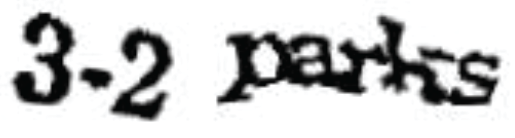
\includegraphics[width=\textwidth]{fig/prior_captcha4.png}\\
                    \center (d) Recaptchas
                \end{minipage}
            }
            \hspace{0.16cm}
            \subfigure{
                \begin{minipage}[t]{0.20\textwidth}
                    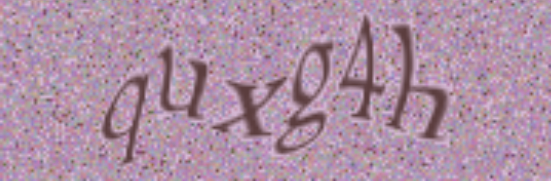
\includegraphics[width=\textwidth]{fig/prior_captcha7.png} \\
                    \center (e) Skyrock
                \end{minipage}
            }
            \hspace{0.16cm}
            \subfigure{
                \begin{minipage}[t]{0.20\textwidth}
                    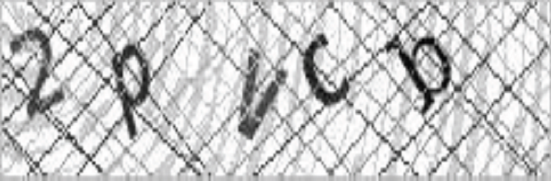
\includegraphics[width=\textwidth]{fig/prior_captcha8.png} \\
                    \center (f) Digg
                \end{minipage}
            }
            \hspace{0.16cm}
            \subfigure{
                \begin{minipage}[t]{0.20\textwidth}
                    
\includegraphics[width=\textwidth]{fig/prior_captcha9.png}\\
                    \center (g) Reddit
                \end{minipage}
            }
            \hspace{0.16cm}
            \subfigure{
                \begin{minipage}[t]{0.20\textwidth}
                    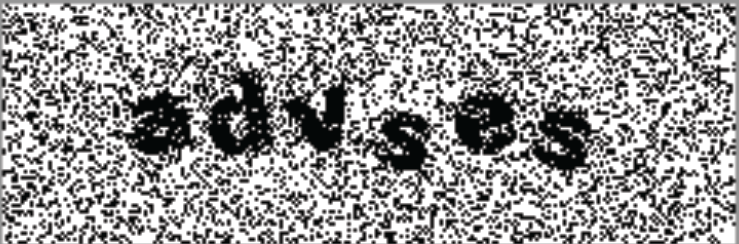
\includegraphics[width=\textwidth]{fig/prior_captcha10.png}\\
                    \center (h) Captcha.net
                \end{minipage}
            }
            \subfigure{
                \begin{minipage}[t]{\textwidth}
                    \center (1) Captchas used in previous attacks.\\
                \end{minipage}
            }
            \hspace{0.16cm}
            \subfigure{
                \begin{minipage}[t]{0.20\textwidth}
                    
\includegraphics[width=\textwidth]{fig/prior_captcha11.jpg} \\
                    \center (i) Tecent
                \end{minipage}
            }
            \hspace{0.16cm}
            \subfigure{
                \begin{minipage}[t]{0.20\textwidth}
                    
\includegraphics[width=\textwidth]{fig/prior_captcha12.jpg} \\
                    \center (j) Baidu
                \end{minipage}
            }
            \hspace{0.16cm}
            \subfigure{
                \begin{minipage}[t]{0.20\textwidth}
                    
\includegraphics[width=\textwidth]{fig/prior_captcha13.jpg}\\
                    \center (k) NetEase
                \end{minipage}
            }
            \hspace{0.16cm}
            \subfigure{
                \begin{minipage}[t]{0.20\textwidth}
                    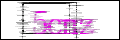
\includegraphics[width=\textwidth]{fig/prior_captcha14.jpg}\\
                    \center (l) VIPSHOP
                \end{minipage}
            }
            \subfigure{
                \begin{minipage}[t]{\textwidth}
                    \center (2) Current Captchas deployed in some popular websites.\\
                \end{minipage}
            }
            \caption{This shows the text-based Captcha schemes used in prior works and current Captchas deployed in some famous websites. The scheme in (a) shows the character isolated Captcha that is deployed originally.}
            \label{fig:text-based captchas}
        \end{figure*}

\textbf{Contributions} This paper makes the following specific contributions:

In order to design a more security Captcha scheme, currently Captchas deployed by many companies 